\documentclass[11pt,a4paper]{article}
\usepackage{graphicx}
\usepackage{alltt}
\usepackage{color}
\usepackage{fancyhdr}
\usepackage{listings}
\usepackage{multicol}
\usepackage{hyperref}
\pagestyle{fancy}
\definecolor{gray_ulisses}{gray}{0.55}
\definecolor{lightgray}{gray}{0.95}
\definecolor{castanho_ulisses}{rgb}{0.71,0.33,0.14}
\definecolor{preto_ulisses}{rgb}{0.41,0.20,0.04}
\definecolor{green_ulises}{rgb}{0.2,0.75,0}
\lstdefinelanguage{HaskellU}
{
	basicstyle=\ttfamily\scriptsize,
	backgroundcolor=\color{lightgray},
	%frameshape={RYRYNYYYY}{yny}{yny}{RYRYNYYYY}, %contornos... muito nice...
	sensitive=true,
	morecomment=[l][\color{gray_ulisses}\scriptsize]{--},
	morecomment=[s][\color{gray_ulisses}\scriptsize]{\{-}{-\}},
	morestring=[b]",
	stringstyle=\color{red},
	showstringspaces=false,
	numbers=left,
	firstnumber=last,
	numberstyle=\tiny,
	numberblanklines=true,
	showspaces=false,
	showtabs=false,
	xleftmargin=10pt,
	xrightmargin=-5pt,
	emph=
	{[2] return,fromJust,readBlockT,writeBlockT,runTransaction,retryTransaction,sequencer,runT,transfer,deposit
,sync,open,close,readBlock,writeBlock,get,put,closeFile,openFile,readB,writeB,flushBuffer	},
	emphstyle={[2]\color{blue}},
	emph=
	{[1] BS,ByteString, TFile,BlockNumber,FT,Maybe,IO,FilePath,Eq,Show,Monad,Handle,Mode,State,TestDisk,Backend,Int
	},
	emphstyle={[1]\color{castanho_ulisses}},
	emph=
	{[3]
		case,class,data,deriving,do,type,else,if,import,in,infixl,infixr,instance,let,
		module,of,primitive,then,type,where,ReadBlock,WriteBlock,Done,Nothing,Just,True,False
	},
	emphstyle={[3]\color{preto_ulisses}\textbf},
	emph=
	{[4] 
	},
	emphstyle={[4]\color{green_ulises}\textbf}
}

\lstnewenvironment{code}[1][]
{\lstset{language=HaskellU,#1}}
{}

\title{ Concurrent Disk-Based Transactions in Haskell}
\author{Satvik Chauhan \and Pankaj More}
\date{{\small \today}}
%
\begin{document}
\maketitle
%
\begin{abstract}
Transactions form an integral part of any multi-user concurrent database system. Most databases implement transactions by various locking mechanism.
In this project, we present a lock free composable file transaction system implemented in a high level functional programming language, Haskell.Our library allows easy composition of transactions and running them as a single atomic transaction thus providing a powerful abstraction in the programmer's tool-kit. The implementation is not only highly concurrent but also non blocking as there are no locks on files. We have exploited the space efficient probabilistic data structure called Bloom Filters to keep primary memory requirements low.


\emph{Keywords:} Concurrency, Transactions, Databases, Haskell

\end{abstract}

%
\section{Introduction}

The major problem in a concurrent system with shared resource is how to share the same resource between all the processes. The traditional way of keeping data consistent is with locks, and we notify threads of changes using condition variables. The example of such mechanism is Haskell's MVar. The drawbacks of using such mechanism is :
\begin{itemize}
\item Race conditions due to forgotten locks
\item Deadlocks resulting from inconsistent lock ordering 
\item Uncaught exceptions resulting in corruption 
\end{itemize}

A transaction is an optimistic way of achieving the same thing without hurting the concurrent part as it allows  all the operations to run concurrently while providing mechanisms to roll-back the resource to a consistent state in case of any failure.

Formally, a transaction is a group of operations combined into a logical unit of work. Developer uses transactions to control and maintain the consistency and integrity of each action in a transaction, despite errors that might occur in the system either due to concurrency or hardware failure. In database context a transaction on a database is considered to be set of operations performed such that database is in a consistent state before and after the transaction and in case of failure the system must provide ways to roll-back partial transactions to bring the database back into a consistent state. Transaction in the database environment mainly serve two purposes:

\begin{enumerate}
\item To provide reliable units of work that allow correct recovery from failures and keep a database consistent even in cases of system failure, when execution stops (completely or partially) and many operations upon a database remain uncompleted, with unclear status.
\item To provide isolation between programs accessing a database concurrently. If this isolation is not provided the programs outcome are possibly erroneous.
\end{enumerate}

Transactions provide an "all-or-nothing" proposition, stating that each work-unit performed in a database must either complete in its entirety or have no effect whatsoever. Further, the system must isolate each transaction from other transactions, results must conform to existing constraints in the database, and transactions that complete successfully must get written to durable storage. Thus, even in case of hardware failure a transaction once commited must persist. A transaction is expected satisfy some guarantees which are often called ACID guarantees: 

\begin{itemize}
\item \emph{Atomicity} means a transaction can end only in two ways: either successfully, in which case all its effects are written to a durable storage and persist between power failures, or unsuccessfully, in which case it has no effect, it can be assumed that this transaction never happened. 
\item \emph{Consistency} just means that a transaction is written correctly, so that when it completes successfully, the database is in a consistent state.
\item \emph{Isolation} means that the transaction appears to execute completely alone, even if, in fact, other transactions are running simultaneously. In other words, transaction always sees a consistent snapshot of the database and is totally unaware of the changes made by other transactions which are running concurrently with it. 
\item \emph{Durability} means that a successful transaction's changes are permanent and persist in all possible sorts of failures. In practice this means to be written on disk. 
\end{itemize}

Software Transactional Memory (STM) is a new way of programming in a shared memory parallel processors. STM gives us a few simple, but powerful, tools with which we can address most of these problems. We execute a block of actions as a transaction using the atomically combinator. Once we enter the block, other threads cannot see any modifications we make until we exit, nor can our thread see any changes made by other threads. These two properties mean that our execution is isolated.Upon exit from a transaction, exactly one of the following things will occur.
\begin{itemize}
\item If no other thread concurrently modified the same data as us, all of our modifications will simultaneously become visible to other threads.
\item Otherwise, our modifications are discarded without being performed.
\end{itemize}

Concurrency in GHC (Glasgow Haskell Compiler) is "lightweight", which means that both thread creation and context switching overheads are extremely low. We can create thousands of threads simultaneously without any problem. Scheduling of Haskell threads is done internally in the Haskell runtime system, and doesn't make use of any operating system-supplied thread packages.

In this library we have tried to imitate and provide similar high-level interface to our transactions library as is provided in case of STM. We will see the example of our interface later.



\section{Lock Based Implementations}
Most of the existing implementations use locks on files for concurrency control. A simplified model of database file locking  is given below.

From the point of view of a single process, a database file can be in one of five locking states:
\begin{itemize}
\item \emph{Unlocked:} No locks are held on the database. The database may be neither read nor written. Any internally cached data is considered suspect and subject to verification against the database file before being used. Other processes can read or write the database as their own locking states permit. This is the default state.
\item \emph{Shared:} The database may be read but not written. Any number of processes can hold shared locks at the same time, hence there can be many simultaneous readers. But no other thread or process is allowed to write to the database file while one or more shared locks are active.
\item \emph{Reserved:}  A reserved lock means that the process is planning on writing to the database file at some point in the future but that it is currently just reading from the file. Only a single reserved lock may be active at one time, though multiple shared locks can coexist with a single reserved lock. Reserved differs from pending in that new shared locks can be acquired while there is a reserved lock.
\item \emph{Pending:}  A pending lock means that the process holding the lock wants to write to the database as soon as possible and is just waiting on all current shared locks to clear so that it can get an exclusive lock. No new shared locks are permitted against the database if a pending lock is active, though existing shared locks are allowed to continue.
\item \emph{Exclusive:} An exclusive lock is needed in order to write to the database file. Only one exclusive lock is allowed on the file and no other locks of any kind are allowed to coexist with an exclusive lock.
\end{itemize}

An example of database engine which follows such model is SQlite.
Multiple readers can read from the database file. 
Only a single writer can write to the database at any given time and all the reader have to wait till the write is complete.
Hence such a model is good for heavy read-based applications but inefficient when multiple write transactions try to modify the database concurrently.

\pagebreak

\section{Algorithm}

\subsection{Simplified version}

We ignore operations other than read and write instructions. We assume that transactions may perform arbitrary computations on data in local buffers in between reads and writes. Our simplified schedules consist of only read and write instructions.

Any transaction has access to following three operations : readblock, writeblock and checkpoint.



\subsection{Hardware Assumptions} FT does not assume that sector writes are atomic . Even though newer disk storage systems guarantee sector writes as atomic using miniature battery based power supply just after a power failure , FT follows a pessimistic approach and assumes that no such facility might be provided by the underlying hardware.

FT assumes that the operating system will buffer writes and that a write request will return before data has actually been stored onto the disk. FT assumes that the flush or fsync will not return until all pending write operations for the file that is being flushed have completed. This assumption might not hold in actual practice. It is possible that the flush and fsync system calls are broken on windows and linux. This is unfortunate as it might lead to data inconsistency during a power failure. However, there is nothing that FT can do to test for or remedy the above situation. The possibility of such scenarios can be reduced by guaranteeing good uptime quality of the hardware.

FT assumes that the detection and/or correction of bit errors caused by cosmic rays, thermal noise, quantum fluctuations, device driver bugs, or other mechanisms, is the responsibility of the underlying hardware and operating system. FT does not add any redundancy to the database file for the purpose of detecting corruption or I/O errors. FT assumes that the data it reads is exactly the same data that it previously wrote.

By default, FT assumes that an operating system call to write a range of bytes will not damage or alter any bytes outside of that range even if a power lose or OS crash occurs during that write. 

\subsection{Commit Workflow}
For maintaining the transaction information and efficient execution of concurrent transactions , we utilize concepts like write ahead logging (WAL) in SQlite, bloomfilters, serializability, etc.

We use bloomfilters to find out rapidly and memory-efficiently, whether a block is present in a journal or not.
A Bloom filter is a space-efficient probabilistic data structure that is used to test whether an element is a member of a set. False positives are possible, but false negatives are not; i.e. a query returns either "inside set (may be wrong)" or "definitely not in set".
Every journal has a corresponding bloomfilter. Bloomfilters instead of indexes are kept in memory to keep memory requirements low and provide good read performance at the same time.
Bloomfilter keeps track of the list of blocks in a journal file.

We store a global queue of committed(valid) journals.

If a transaction is purely read-based , it need not keep any journal. 
If the transaction is in ReadWrite Mode , it will have its own journal. 

ReadBlock first tries reading from its own journal if it exists. Then it tries to read from the queue of commited journals. It doesnt actually need to perform I/O on every journal to find the block. It checks the bloomfilter associated with each journal and if bloomfilter reports true , it actually performs I/O to find out if it is true. As a side note, it is obvious that the goal is to minimize the false rate positive of bloomfilter so that such costly disk accesses can be minimized. Proper real time benchmarking and fine-tuning of bloom filter parameters can reduce false-positive rate and optimize the performance. If it really finds the block , then it fetches the data from the disk and returns it. If the bloomfilter had signalled a false-positive , it needs to continue its search further down the queue recursively. If the queue is fully traversed and the block is not found , it finally reads from the main database file. 
 
WriteBlock simply writes the block data to its own journal file. It might latter fail to commit if there are conflicts. This is discussed below.

When a transaction needs to commit , it first checks whether there is a conflict between the blocks that it read and the blocks changed between the file version when it started and the current file version. If a conflict exists , the transaction must abort. If there are no such conflicts and it was a read only transaction then it commits successfully. Whereas,  in case of a read-write transaction , it adds its journal to the journal queue with the incremented file version. It also increments the file version of the main database file. It flushes the required buffers so that the data gets actually written to the disk to guarantee durability.




\subsection{Acid Guarantees}
\begin{itemize}
\item Atomicity: 
    Transaction either commits or aborts.
\item Consistency: 
    The set of valid journals and transaction file is always consistent
\item Isolation: 
	Since the journal of a concurrently running transaction is not yet valid(as it is not yet committed) , the journal must not be in the global journal queue. Hence , a concurrent transaction can never see the change made by another running transaction.
\item Durability: 
    Once a transaction commits , fsync must ensure that the data is actually written onto the disk. Hence assuming our calls to fsync are always called at the appropriate time , the burden of durability rests on the fsync system call correctness in the host operating system.
\end{itemize}

\subsection{Sequencer}
If there are large number of transactions executing concurrently , the number of journals can grow large extremely fast. There is a need to keep the number of journals in control else it would lead to extremely bad read performance. A checkpoint operation transfers all the data in journal files to the main database file. Hence , frequent checkpointing would reduce the overhead of read operations.

\subsection{Read-write Trade-off}
There is a trade-off between average read performance and average write performance. To maximize the read performance, one wants to keep the number of journal files as small as possible and hence run checkpoints frequently. To maximize write performance, one wants to amortize the cost of each checkpoint over as many writes as possible, meaning that one wants to run checkpoints infrequently and let the no of journal files grow as large as possible before each checkpoint. The decision of how often to run checkpoints may therefore vary from one application to another depending on the relative read and write performance requirements of the application.



\pagebreak
\section{Implementation Details}

Here we will explain some important parts of our implementations which are directly taken from the lhs files. The explanation is in the blog style of writing.

Lets try to capture the transaction into a data-type first. Here
we are implementing a very basic version of transactions. So our
transaction system only provide two type of operations to be performed
on the file.

\begin{enumerate}
\item \textbf{ReadBlock} is to read the data from the given block number.
\item \textbf{WriteBlock} is to write the given data on the block number provide.
\end{enumerate}

We can also think of adding operations like append block, modify block
etc., but to keep it simple we only support these two basic operations.
Now lets look at the data definition of the File Transaction (FT) data
type.

\begin{code}[name=Transactions]
-- Transactions.lhs
-- | Transaction Datatype
data FT a = 
    Done a | 
    ReadBlock BlockNumber (BS.ByteString -> FT a) | 
    WriteBlock BlockNumber BS.ByteString (FT a)
\end{code}

ByteString is made explicit as all the data needs to be serialized to ByteString before writing.
The types of ReadBlock and WriteBlock looks a little odd. We will see later how it helps in actually passing the continuations.
Lets see the monad definiton of the FT datatype.

\begin{code}[name=Transactions]
-- Transactions.lhs
-- | Monad Definition for the Transaction. 
instance Monad FT where 
    return = Done 
    m >>= f = case m of 
        Done a -> f a 
        ReadBlock bn c -> ReadBlock bn (\i -> c i  >>= f) 
        WriteBlock bn x c -> WriteBlock bn x (c >>= f)
\end{code}

Here we will see how the types of ReadBlock and WriteBlock actually help
in our continuation passing style of programming. Lets see a simple
example of interface our implementation provides.
Consider the famous banking example for transactions. We want to
transfer x fund from account A to account B.
Lets assume that fund informations of A and B are stored in the same
file at block number a and b respectively.
First we will see the basic example to deposit amount to an account. 
Here is a function which deposits x amount to the given account. 

\begin{code}
deposit a x = do 
      amount <- ReadBlock a return 
      WriteBlock a (amount + x) (return ())
\end{code}

Lets see how this is translated to explicit notation without do
notation.

\begin{code}[stepnumber=2]
 ReadBlock a return >>= (\amount -> WriteBlock a 
   (amount +x) (return()))
 ReadBlock a (\i -> return i >>= 
   \amount -> WriteBlock a (amount + x) (return()))
 ReadBlock a (\i -> Done i  >>= 
   \amount -> WriteBlock a (amount + x) (return()))
 ReadBlock a (\amount -> 
   WriteBlock a (amount + x) (return()))
\end{code}

Looks like it got transformed to whatever we wanted. This is how continuation passing style actually works.
It was a little frustrating to write return while writing ReadBlock and
WriteBlock. So lets define some helpers to help us avoiding the
repetitions.

\begin{code}[name=Transactions]
-- Transactions.lhs
-- | readBlockT to be used inside the FT Monad 
readBlockT :: BlockNumber -> FT BS.ByteString
readBlockT = flip ReadBlock return 
-- | writeBlockT to be used inside the FT Monad 
writeBlockT :: BlockNumber -> BS.ByteString -> FT ()
writeBlockT v x =  WriteBlock v x $ return () 
\end{code}

Now the above deposit function can easily be written as:

\begin{code}
deposit a x = do 
      amount <- readBlockT a 
      writeBlockT a (amount + x)
\end{code}

Now we want to actually perform the transactions satisfying all the ACID
guarantees. So we need to write a function to actually convert our
Transactions from FT monad to IO monad and perform them.
According to the semantics of a transaction, a transaction can either
fail or succeed. So we should provide atleast two types of functions to
run a transaction which are as follows:

\begin{code}[name=Transactions]
-- Transactions.lhs
-- | Runs the given transaction on the file. 
-- Transaction may fail in which case it returns Nothing.
runTransaction :: FT a -> TFile -> IO (Maybe a)
runTransaction = runT Nothing False
-- | Runs the transaction on the file. 
-- If transaction fails then reruns it
-- with higher priority.
retryTransaction :: FT a -> TFile -> IO a
retryTransaction ft tFile = fromJust <$> 
	runT Nothing True ft tFile 
\end{code}

At this point before implementing anything else we are interested in how
we will be actually using them. Here I will also introduce you to the
power of composing two transactions and running them as one. Lets
comeback to our backing example.

\begin{code}[name=Transactions]
transfer a b x = do 
  deposit a (-x) 
  deposit b x
\end{code}

Here is the function to remove x amount from account A and deposit it to
the account B. We have implemented a very loose semantics here as to not
check if A's balance is less than 0 etc.. I just wanted to show the power
of composing functions. Now we can just do runTransaction on transfer to
run this transaction.

\begin{code}[name=Transactions]
-- Transactions.lhs
runTransaction (transfer a b 100)
\end{code}

The semantics of runTransaction automatically
takes care of all the possible failures and roll-back in case of
transaction failure.

runTransaction actually has to take care of lots of things:

\begin{itemize}
\item Gets the file Version at which the transaction started.
\item Performs the transactions on the Journal File 
\item Then tries to commit the transaction.Checks the present version against the version at which it started. Here comes the idea of space efficient Bloom filters which are actually used to check whether the current transaction should commit successfully or not. This operation is in a critical section as it might leave the file in inconsistent state if it is not isolated. 
\item return the output if transaction succeeds otherwise adds the failed transactions to the failed queue. If retryTransaction was used then it again tries to perform the transaction. 
\end{itemize}

All the journals of the transactions get aggregated over time which might result in poor read performances over time. So we need to actually checkpoint the committed journals back to the database file.

\begin{code}[name=Transactions]
-- Transactions.lhs
sequencer :: TFile -> IO () 
\end{code}

Sequencer actually does this. It checks for the committed journal files, writes them to the actual database and removes them. 

\section{Future Improvements}
None of the implementation is good for all the purposes. This implementation is good when we have lots of not colliding write transactions. If too many transaction collide and fail then we get poor concurrency. Thus other goal would be to add locking transactions which actually perform the write transactions sequentially similar to sqlite. 
Other step will be in the direction of heavily testing the implementation. As it is always very difficult to test alone concurrent applications, we on the other hand also have lots of file operations. The quickcheck library in Haskell provides very good testing mechanism but it requires to separate the backed from the IO monad and to provide an abstraction over it.
Here is our basic approach of creating a pure interface to IO which actually don't perform IO but simulate the file-system. 

Here the basic idea is to capture the Backend in a typeclass. We will be exploiting the type-families extension of Haskell to separate backend from the actual transaction implementation. This has great advantage to replace our backend with whatever kind we want.

\begin{code}[name=Backend,firstnumber=1]
-- Backend.hs
class (Show a,Monad m) => Backend b m a | b -> m where 
    data Handle :: * -> * 
    type BlockNumber :: *  
    open :: FilePath -> Mode -> m (Handle b)
    close :: Handle b -> m () 
    readBlock ::(Eq BlockNumber)=>Handle b->BlockNumber->m a 
    writeBlock ::(Eq BlockNumber)=>Handle b->BlockNumber->a->m ()
    sync :: Handle b -> m ()
\end{code}

We have added the basic functions which we need in the transaction implementation. This greatly condense the side effects possible to only these functions.

Here is the pure implementation of the file system in terms of state monad. 

\begin{code}[name=Backend,firstnumber=last]
-- Backend.hs
instance Show a => Backend (TestDisk a)  (State (TestDisk a)) a where 
    data Handle (TestDisk a) = Handle FilePath 
    type BlockNumber = Int 
    open fp m = do 
        disk <- get
        put $ openFile disk fp m 
        return $ Handle fp
    close (Handle fp) = do 
        disk <- get 
        put $ closeFile disk fp
    readBlock (Handle fp) bn = do 
        t <- get 
        case readB t fp bn buffers of 
            Nothing -> error "Block Not Found"
            Just a -> return a
    writeBlock (Handle fp) bn a = do 
        t <- get 
        put $ writeB t fp bn a 
    sync (Handle fp) = do  
        t <- get 
        put $ flushBuffer t fp
\end{code}

Such an implementation allows us to test lots of the properties which are otherwise difficult to test. It also helps in explicitly specifying what kind of expectation and assumptions you make on your backend.

The very simple representation of the disk simulated as a map between FilePath and File. 
We also have buffers to simulate sync. This will help to simulate power failures and hardware crashes as the data present in the buffers are lost but not the disk. \\
The File representation is very simple. Just a map between block number and the data present at that location.

\begin{code}[name=Backend]
-- Backend.hs
data TestDisk a = TestDisk {
    disk :: M.Map FilePath (File a)
   , buffers :: M.Map FilePath (File a) 
   , bufferSize :: Int -- Current buffer Size 
   , openFiles :: M.Map FilePath Mode
    } deriving (Eq,Show)
data File a = File {
    blocks :: M.Map Int a 
   , size :: Int 
    } deriving (Eq, Show)

data Mode = ReadWrite | Read | Write deriving (Eq,Show) 
\end{code}

This was a very basic structure of file system which we will be using to write test-cases using quick check. Another major thing left to abstract is concurrency and IORefs. This will be our next focus of work in the future. Another area of focus will be into optimizing the implementation and comparing its performance with sqlite. This will greatly improve our understanding whether Haskell is suitable for writing industrial strength databases. 


\bibliographystyle{IEEEbib}
\begin{thebibliography}{10}
\bibitem[1]{stm}Anthony Discolo, Tim Harris, Simon Marlow, Simon Peyton Jones, and Satnam Singh. Lock-free data structures using STMs in Haskell. In Eighth International Symposium on Functional and Logic Programming (FLOPS’06), April 2006.
\bibitem[2]{sqlite}Atomic Commit in sqlite, \url{http://www.sqlite.org/atomiccommit.html}
\bibitem[3]{bloomfilter}Bloom Filter, \url{http://en.wikipedia.org/wiki/Bloom_filter}
\bibitem[4]{WAL}Write-Ahead Logging, \url{http://www.sqlite.org/draft/wal.html}
\end{thebibliography}

\pagebreak



\begin{figure}[htb]
\centering
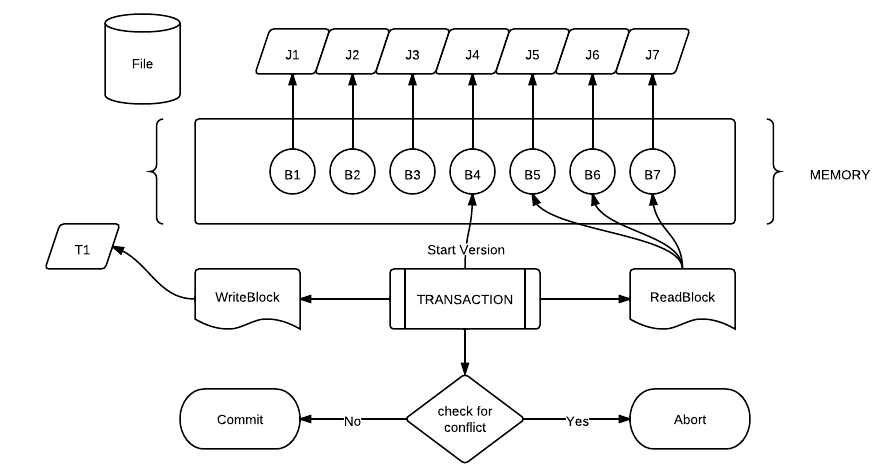
\includegraphics[angle=90]{1}
\end{figure}

\pagebreak

\begin{figure}[htb]
\centering
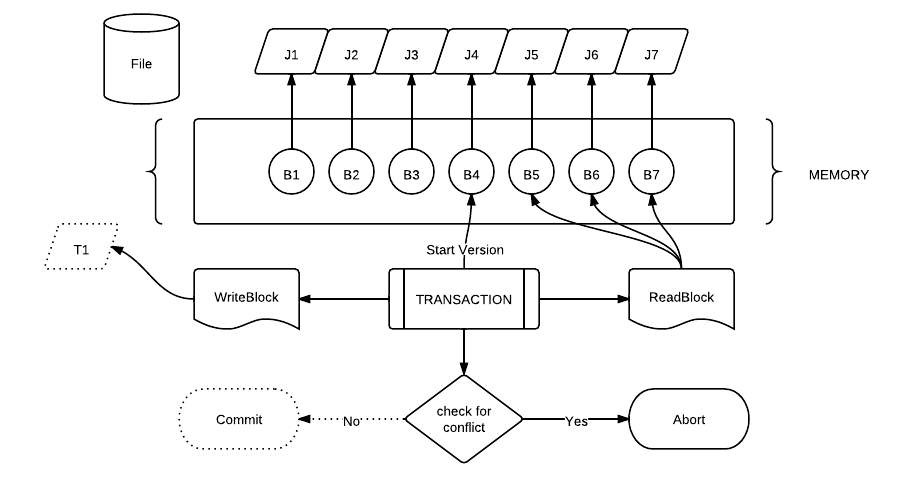
\includegraphics[angle=90]{2}
\end{figure}

\pagebreak

\begin{figure}[htb]
\centering
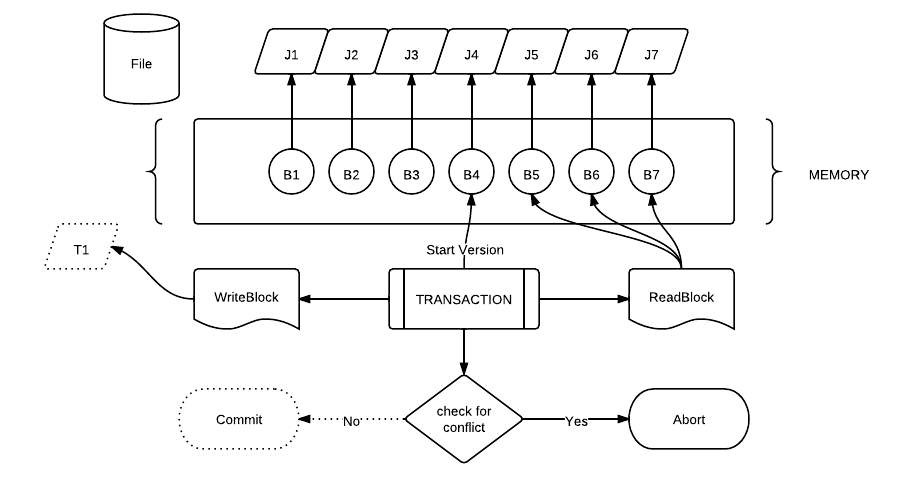
\includegraphics[angle=90]{2}
\end{figure}

\pagebreak

\end{document}
